% !TeX spellcheck = it_IT
\newpage
\section{Memorie}
Una memoria avrà:
\begin{itemize}
	\item Indirizzo da leggere, $k$ bit
	\item Indirizzo dove scrivere, $k$ bit
	\item Cosa scrivere, $n$ bit
	\item Write Enable, $1$ bit
	\item Valore letto, $n$ bit
\end{itemize}
\begin{center}
	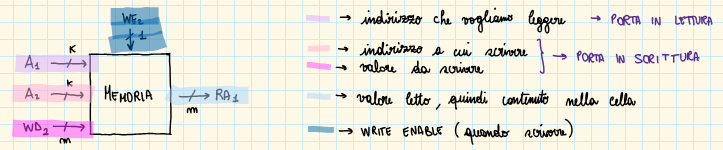
\includegraphics[scale=.6]{memoria}
\end{center}

\subsection{RAM}
Le memorie ad accesso casuale forniscono un tempo di accesso equivalente ad ogni cella.
\subsubsection{DRAM}
È una memoria \textbf{dinamica}, ovvero ha sempre bisogno di essere rinfrescata in quanto è composta da condensatori che mantengono la carica per un tempo limitato.\\
Quando eseguiamo una lettura il dato passa dal condensatore alla linea di bit e di conseguenza viene perso e ha bisogno di essere refreshato. Viceversa per quando scriviamo.
\begin{center}
	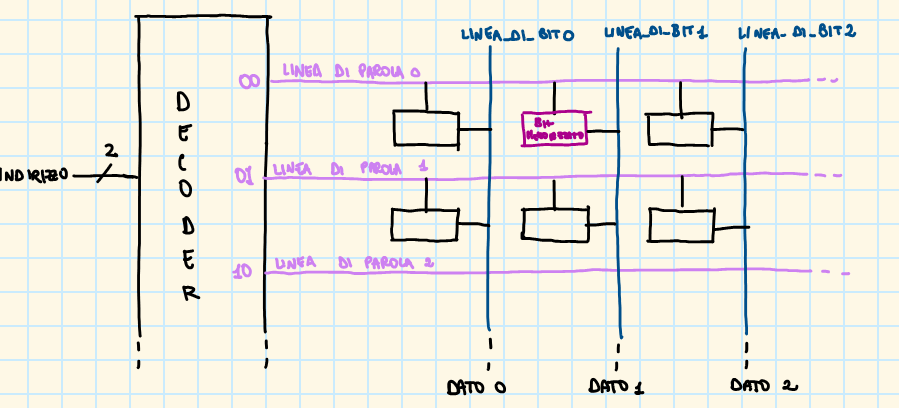
\includegraphics[scale=.3]{dram}
\end{center}

\subsubsection{SRAM}
A differenza delle DRAM utilizziamo più transistor ma questo ci permette di evitare l'operazione di refresh.
\begin{center}
	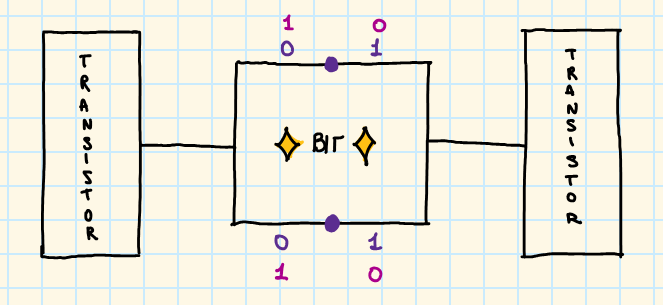
\includegraphics[scale=.3]{sram}
	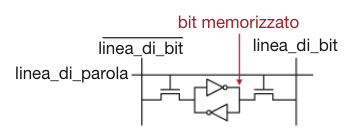
\includegraphics[scale=.4]{sram2}
\end{center}

\subsection{ROM e PROM}
La Read Only Memory è una memoria non volatile in sola lettura, strutturata in maniera molto simile alla DRAM e SRAM, con linee di parola, transistor e condensatori.\\
La \textbf{PROM} è una ROM programmabile, dove il programmatore può decidere i valori e poi salvarli bruciando i fusibili connessi alle celle di memoria.

\subsection{Memorie modulari}
Questo approccio alla progettazione di memoria prevede una mappatura in moduli più piccoli. La decomposizione può avvenire in due modi:
\begin{itemize}
	\item \textbf{Orizzontale}
	\begin{itemize}
		\item \textbf{Sequenziale}: date $n$ celle e $c$ moduli, dividiamo in $\frac{n}{c}$. Per cercare i dati usiamo poi i bit più significativi dato che i moduli posseggono un solo blocco
		\item \textbf{Interlacciata}: classifichiamo un bit si ed uno no, favorendo il parallelismo e diminuendo il costo di accesso
	\end{itemize}
	\item \textbf{Verticale}
\end{itemize}

\subsection{Memoria associativa}
In questo tipo di memoria associamo $k$ chiavi a $k$ locazioni nel momento in cui questa viene occupata da un valore. Nel momento in cui abbiamo una \textbf{hit} vuol dire che esiste quella chiave in memoria e possiamo cercarla.
\begin{center}
	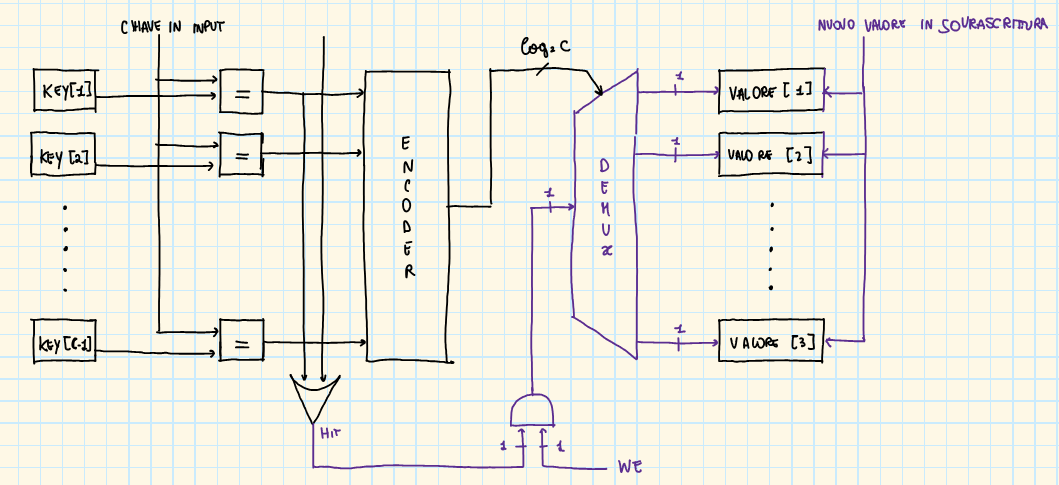
\includegraphics[scale=.4]{associativa}
\end{center}